

\chapter{Comparison}
This chapter focus on the comparison of our implementation with existing other implementation in MobilityDB.  In this section, the algorithms implemented in MobilityDB and SQUISH-E will be compared on various measures. Essentially performance and similarity, the competition factor will also be derived in order to determine whether the SQUISH-E points at the output compete with the algorithms present when we duplicate them. Tests and results are retrieved through MobilityDB and processed from a custom front-end under react and grafana to obtain an analytical dashboard. Comparisons will only be made between versions implemented in MobilityDB.


\section{Douglas-Peucker}

As mentioned in the state of the art Douglas-Peucker is a trajectory simplification algorithm based on offline execution. So it needs the full trajectory in order to work properly.

\subsection{Performance}
The executions were run under different point sizes by varying the input parameters. The lambda variables were chosen to approximate compression ratios between 90\%-1\%. The points have no real geographical position and are in fact at the same location, in order only to underline the performance of the .

\begin{table}[htbp]
    \centering
    \label{tab:execution_time_douglas}
    \begin{tabular}{@{}lccccc@{}}
        \toprule
        Number of Points & \multicolumn{5}{c}{Lambda} \\
        \cmidrule{2-6}
        & 5         & 2       & 0.02        & 0.002       & 0.0002       \\
        \midrule
        100              & 00.000075 & 00.000107 & 00.000691 & 00.000581 & 00.000606 \\
        1000             & 00.00019  & 00.000194 & 00.056759 & 00.055591 & 00.056859 \\
        10000            & 00.001531 & 00.001675 & 05.721065 & 05.798434 & 05.600994 \\
        100000           & 00.017149  & 00.013302  & EOF & EOF & EOF \\
        1000000          & 00.169507 & 00.147934 & EOF & EOF & EOF \\
        \bottomrule
    \end{tabular}
    \caption{Average Execution Time by Number of Points and Distance}
\end{table}

The table \ref{tab:execution_time_douglas} shows the results representing the number of input points and the lambda parameter given to Douglas-Peucker.
It's quite astonishing to see the speed of the algorithm for lambda=5. Having a speed higher than an execution on C while the program runs under psql.  This is due to the nature of Douglas-Peucker, which doesn't continue with unnecessary simplifications and starts with the extremities. We can also see that for values less than or equal to 0.02 the algorithm is quite slow and even causes EOFs. We can point out that to have simplifications at a rate of less than 50\% Douglas-Peucker is quite fast, but when the compression must be above a certain threshold which depends on any trajectory as the parameter is an error distance and not a compression rate then it becomes quite slow compared to its sibling SQUISH-E.  SQUISH-E is fairly constant and is the slowest for a compression ratio of 50\% as seen above.

\subsection{Similarity}
Similarity is an important measure for comparing these two algorithms with two different inputs, so in order to make a comparison let's look at the level of compression at the output. 


\begin{table}[htbp]
	\centering
	\label{tab:douglas_vs_squish_comparison}
	\begin{tabular}{@{}lccc@{}}
		\toprule
		& \multicolumn{3}{c}{\textbf{Douglas}} \\
		\cmidrule(l){2-4}
		\textbf{SquishE} & 0.02 & 0.002 & 0.0002 \\
		\midrule
		\textbf{1x} 	& 18 	& 67 & 768 \\
		Frechet 		& -3015 & -3215 & -617.274 \\
		Hausdorff 		& -3015 	& -3215 & -617.274 \\
		DTW 			& -90073593 	& -15597514 & -5325534 \\
		Temporal 		& 1899 	& 129.712 & 1.397 \\ \midrule
		\textbf{2x} 	& 36 & 134 & 1536 \\
		Frechet 		& -28363 & -6034 & -617.274 \\
		Hausdorff 		& -28363 & -6034 & -617.274 \\
		DTW  		& -262452925 & -47034601 & -8163405 \\
		Temporal 	& 102 & 19.191 & -1.590 \\ \midrule
		\textbf{3x} 	& 54 & 201 & 2304 \\
		Frechet 		& -34532 & -8073 & -617.274 \\
		Hausdorff 		& -34532 & -8073 & -617.274 \\
		DTW 		& -299629282 & -60327008 & -9036166 \\
		Temporal 			& -149 & -12.72 & -1.933 \\ \midrule
		\textbf{4x} 	& 72 & 268 & 3072 \\
		Frechet 		& -36615 & -10146 & -617.274 \\
		Hausdorff 		& -36615 & -10146 & -617.274 \\
		DTW 		& -325049247 & -65978902 & -9504295 \\
		Temporal 			& -278 & -22.036 & -2.315 \\
		\bottomrule
	\end{tabular}
	\caption{Comparison of differences between Douglas and SquishE (Frechet, Hausdorff, DTW)}
\end{table}

The table \ref{tab:douglas_vs_squish_comparison} shows the differences in distances between the two algorithms. The different boxes represent the number of points SQUISH-E outputs compared to Douglas.
Note that if the result is negative, SQUISH-E is more accurate than Douglas. For spatial distances such as Frechet and Hausdorff, we can see that SQUISH-E with the same number of points is more accurate. SQUISH-E, on the other hand, has a larger temporal area than Douglas, which shows that SQUISH-E's gap areas are larger than Douglas's, and competes with Douglas at x3 for small percentages, but x2 when the number of points is larger.



\section{MinDist}
\subsection{Performance}
Min distance is a second algorithm implemented in MobilityDB. Min distance, like douglas, works offline and requires the entire trajectory in order to run correctly. % à décrire dans l'état de l'art
\begin{table}[htbp]
    \centering
    \label{tab:execution_time_mindist}
    \begin{tabular}{@{}lccccc@{}}
        \toprule
        Number of Points & \multicolumn{5}{c}{Lambda} \\
        \cmidrule{2-6}
        & 5         & 2       & 0.02        & 0.002       & 0.0002       \\
        \midrule
        100              & 00.000021 & 00.000006 & 00.000023 & 00.000014 & 00.000016 \\
        1000             & 00.000041  & 00.000036 & 00.00012 & 00.00012 & 00.000123 \\
        10000            & 00.000291 & 00.000293 & 00.001307 & 00.00134 & 00.001449 \\
        100000           & 00.003088  & 00.003044  & 00.015219 & 00.015609 & 00.016354 \\
        1000000          & 00.034338 & 00.036202 & 00.152152 & 00.163061 & 00.178996 \\
        \bottomrule
    \end{tabular}
    \caption{Average Execution Time by Number of Points and Distance of MinDist Algorithm}
\end{table}

In terms of performance, min distances outperforms SQUISH-E. Min distance is slower when we increase the lambda variable.

\subsection{Similarity}
As in the previous section, the table below shows the similarity comparison between min distance and SQUISH-E.

\begin{table}[htbp]
	\centering
	\label{tab:mindist_vs_squish_comparison}
	\begin{tabular}{@{}lccc@{}}
		\toprule
		& \multicolumn{3}{c}{\textbf{Mindist}} \\
		\cmidrule(l){2-4}
		\textbf{SquishE} & 0.02 & 0.002 & 0.0002 \\
		\midrule
		\textbf{1x} 	& 418 	& 3652 & 16919 \\
		Frechet 		& 2842.859 & 582.269 & 33.645 \\
		Hausdorff 		& 2842.859 	& 582.269 & 33.645 \\
		DTW 			& 1834655 	& 95109 & 21682 \\
		Temporal 		& 1.54 	& 0.158 & 0.091 \\ \midrule
		\textbf{2x} 	& 836 & 134 & ALL \\
		Frechet 		& 598.393 & 582.269 & -66.409 \\
		Hausdorff 		& 598.393 & 582.269 & -66.409 \\
		DTW  		& -3452102 & -463775 & -36834 \\
		Temporal 	& -3.687 & -0.563 & -0.647 \\ \midrule
		\textbf{3x} 	& 1254 & 201 & // \\
		Frechet 		& 598.393 & 582.269 &  // \\
		Hausdorff 		& 598.393 & 582.269 &  // \\
		DTW 		& -5014557 & -655462 &  // \\
		Temporal 			& -4.926 & -1.192 & // \\ \midrule
		\textbf{4x} 	& 1672 & 268 &  // \\
		Frechet 		& 598.393 & 582.269 &  // \\
		Hausdorff 		& 598.393 & 582.269 &  // \\
		DTW 		& -5960279 & -768674 &  // \\
		Temporal 			& -5.538 & -1.764 &  // \\
		\bottomrule
	\end{tabular}
	\caption{Comparison of differences between MinDist and SquishE (Frechet, Hausdorff, DTW)}
\end{table}

We can see in \ref{tab:mindist_vs_squish_comparison} and observe that min distance is remarkably accurate. SQUISH-E competes with min distance for double the number of points in output, but is less accurate for spatial metrics such as fréchet and Hausdorff. min distance has a surprising combination of performance and accuracy. SQUISH-E's advantage over min distance is its ability to operate in a streaming environment. We can also note that SQUISH-E competes with min distance when the number of points is multiplied by 2 in spatiotemporal metrics such as DTW and temporal.


\section{DashBoard}

To get a more global view and a picture of the comparison here are some graphs that can be obtained from the dashboard data: 


\begin{figure}[!h]
	\centering
	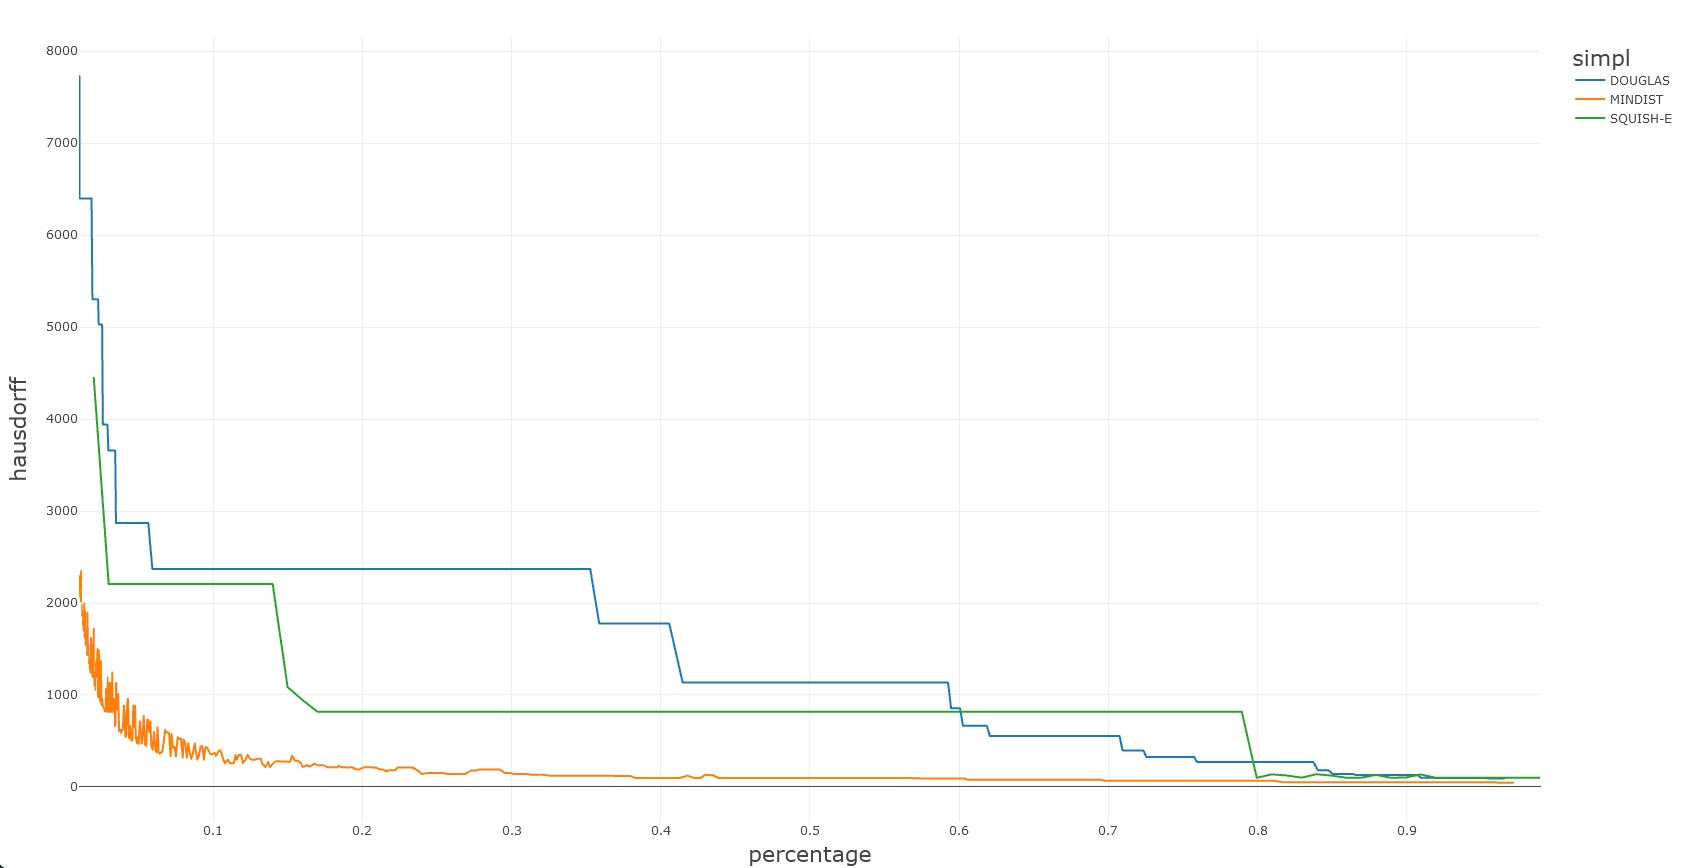
\includegraphics[width=1\linewidth]{figures/Stats/hausdorff_comp.jpg}
	\caption{Hausdorff comparison}
	\label{fig:comp_h}
\end{figure}


\begin{figure}[!h]
	\centering
	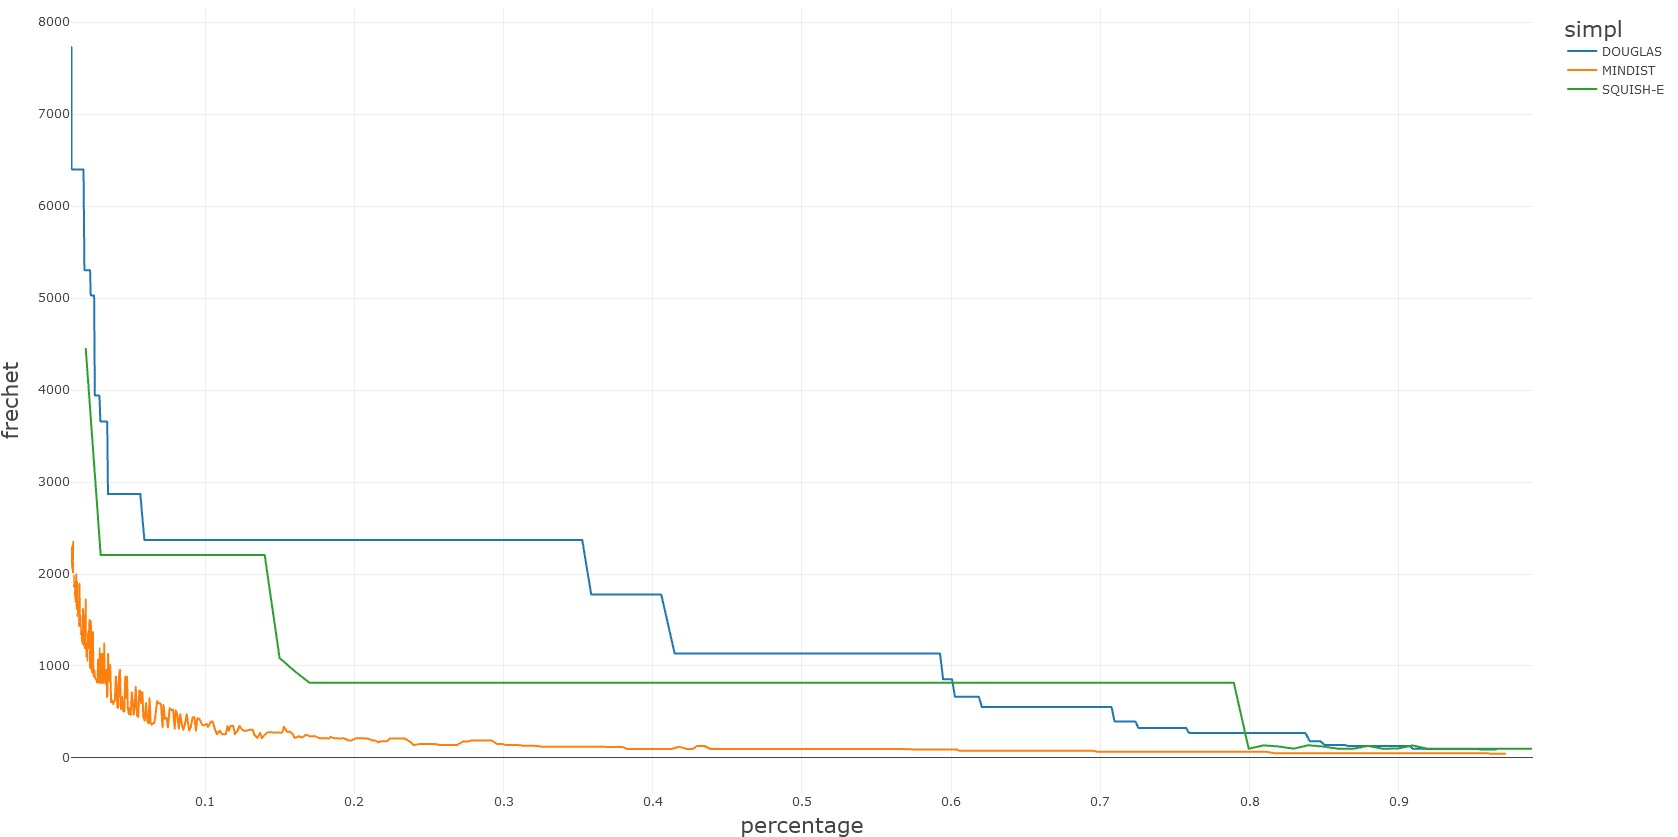
\includegraphics[width=1\linewidth]{figures/Stats/frechet_comp.jpg}
	\caption{Frechet comparison}
	\label{fig:comp_f}
\end{figure}


\begin{figure}[!h]
	\centering
	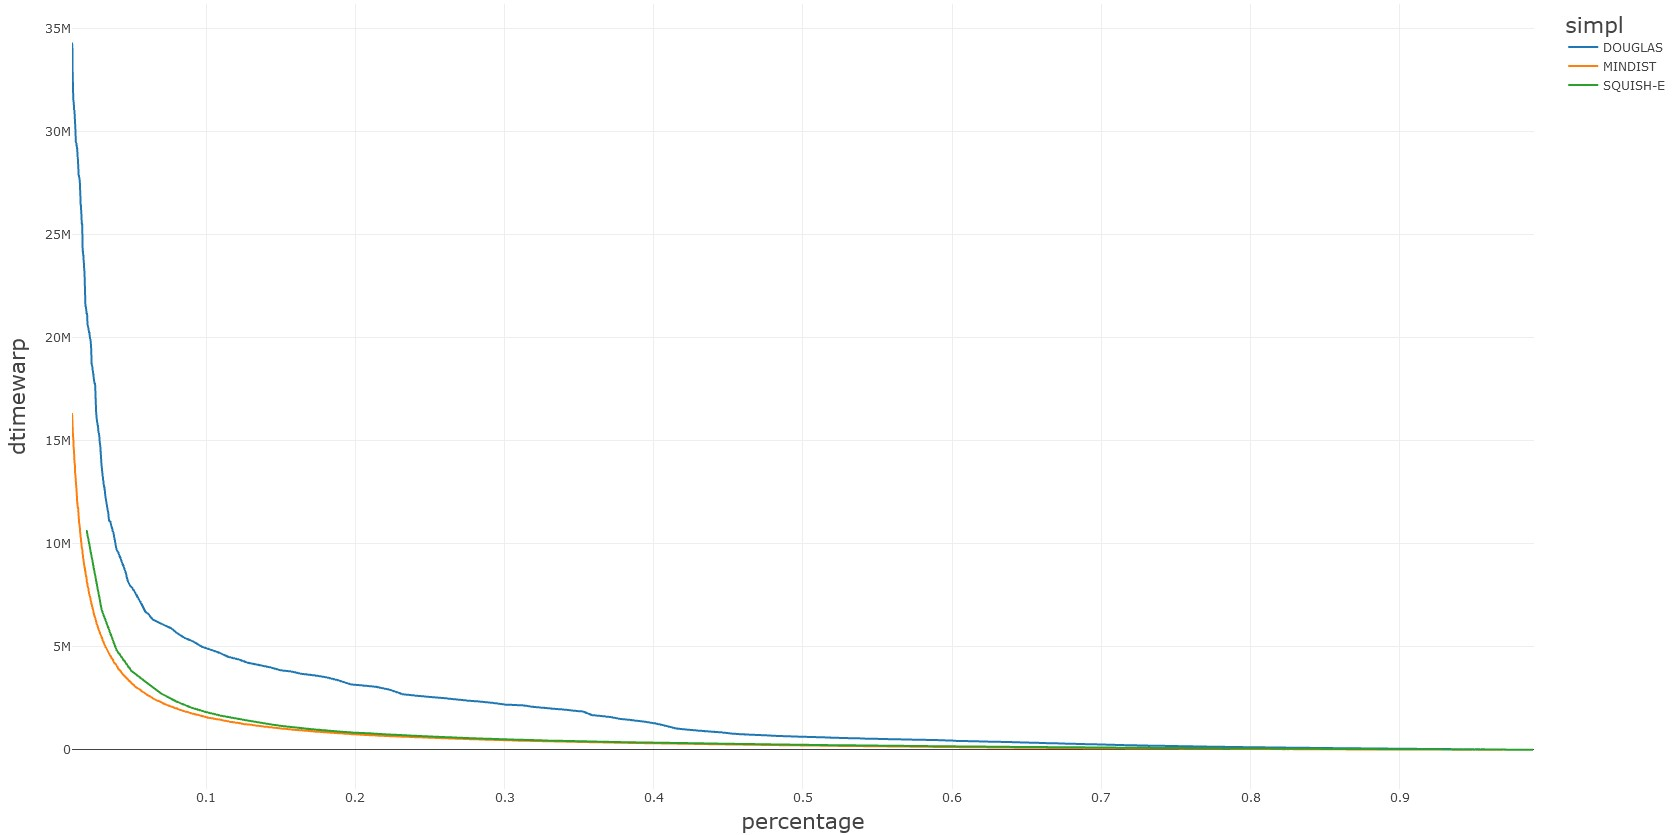
\includegraphics[width=1\linewidth]{figures/Stats/dtw_comp.jpg}
	\caption{DTW comparison}
	\label{fig:comp_dt}
\end{figure}


\begin{figure}[!h]
	\centering
	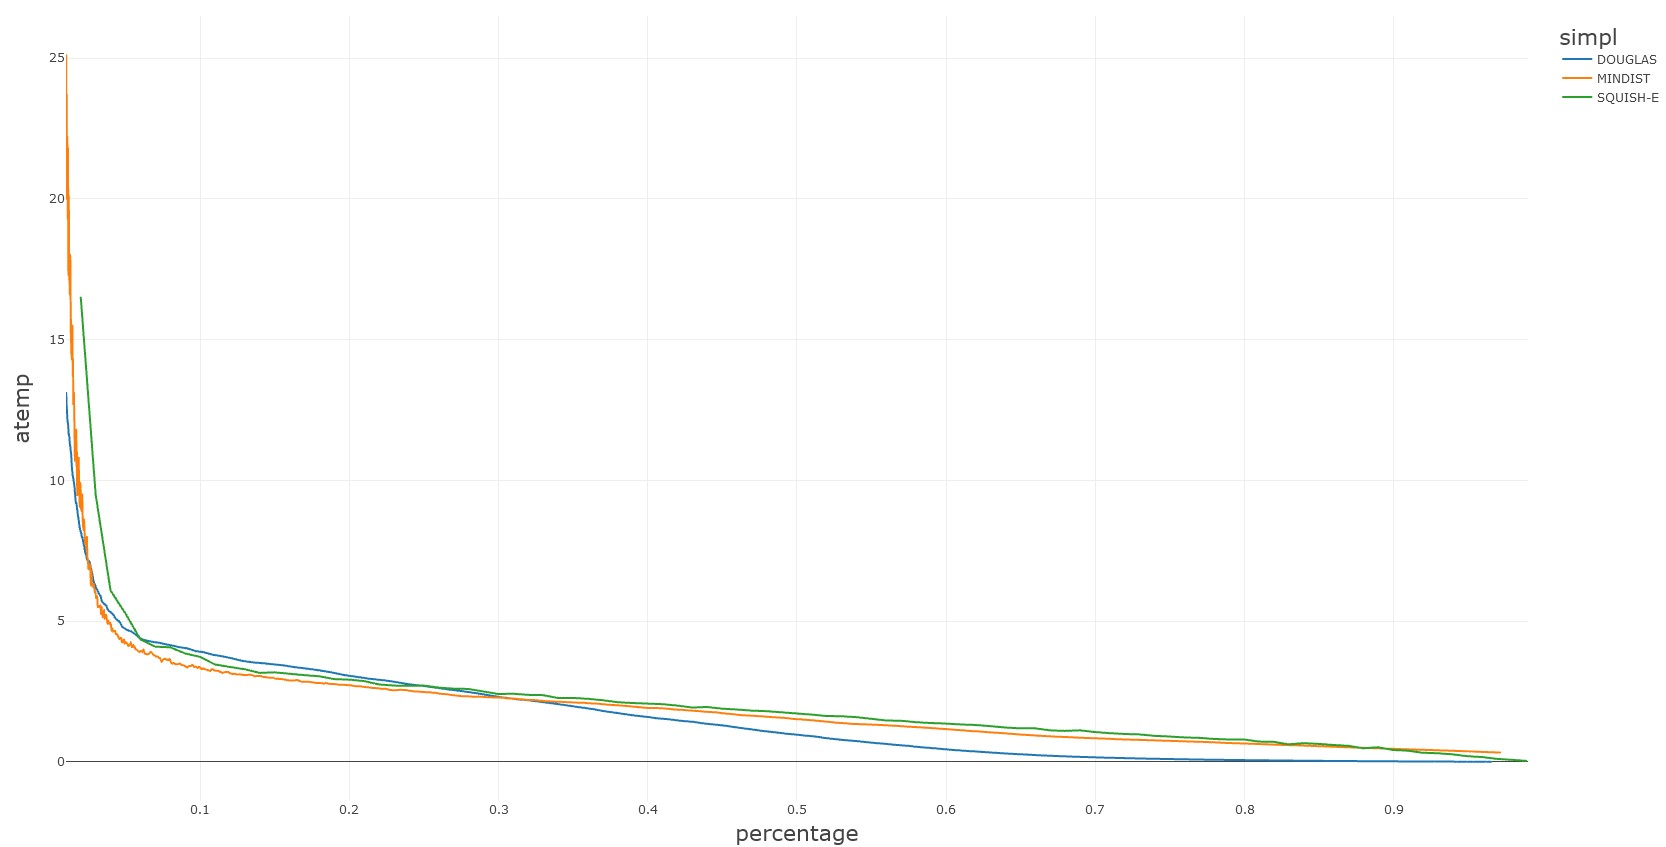
\includegraphics[width=1\linewidth]{figures/Stats/atemp_comp.jpg}
	\caption{Temporal Integral comparison}
	\label{fig:comp_at}
\end{figure}

These figures show the comparison of accuracies on trajectory 1 between the three algorithms mentioned above (Douglas,SQUISH-E,MinDist). Here the variation in error distance as a function of compression level can be observed. Frechet and Hausdorff's error level for Douglas and SQUISH-E has a staircase formation, while for Mindistance it constantly decreases. SQUISH-E is generally better than douglas and worse than min distance, except in \ref{fig:comp_at} where SQUISH-E is worse but very close to its competitors.
